\documentclass{beamer} 

\usepackage{graphicx}
\usepackage{subfigure}

%\usepackage{xeCJK} % 中文包
\usetheme{Boadilla}  
\usecolortheme{seagull} 

%\setbeamertemplate{caption}[numbered] % 序号
%\setbeamercovered{transparent=15}
\setbeamersize{text margin left=0.6cm, text margin right=0.6cm} % 设置页边距
\setbeamercovered{transparent} 
\setbeamertemplate{navigation symbols}{} %Navigationsleiste ausschalten     


\title{Weekly work summary}
\author{Guangzhi Ren}
\institute {}
\date{\today}

%============================================================
\begin{document}

\begin{frame}
\titlepage   
\end{frame}

\begin{frame}{content}
	\begin{itemize}
%		\item references on electromagnetic turbulence
		\item comparision between different algorithm
		\item revisiting to former simulation result
		\item modification of energy transfer equation 
		\item ZF/RHF/GAM	
\end{itemize}
\end{frame}
	

\begin{frame}{comparision between different algorithm}
\begin{figure}[H]
	\centering
	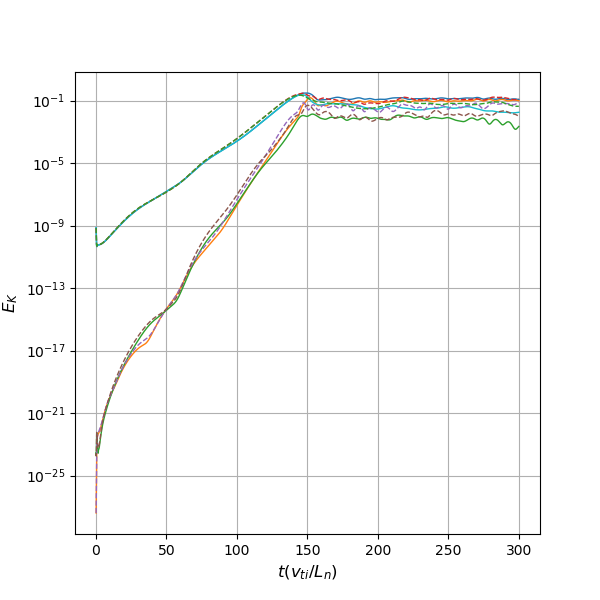
\includegraphics[width=0.5\textwidth]{./images/ek-256.png}
	\caption{time evolution of energy in LW/RK/AB}
\end{figure}
\end{frame}	
	
\begin{frame}{comparision between different algorithm}
\begin{figure}[H]
	\centering
	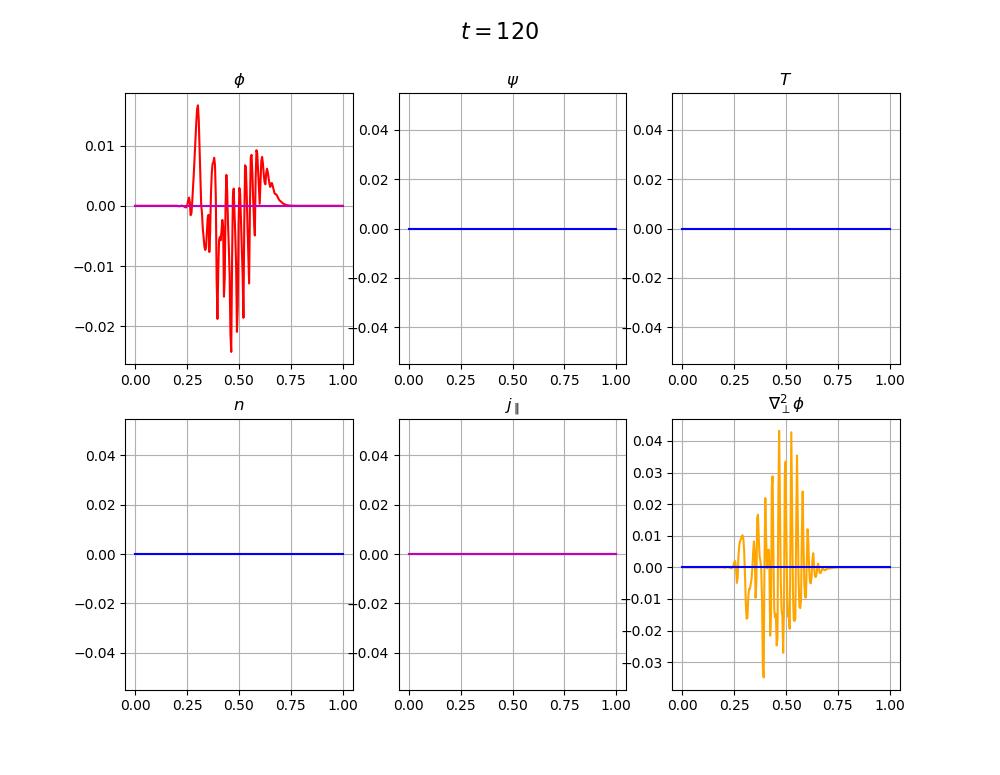
\includegraphics[width=0.7\textwidth]{./images/ab-256-120.png}
	\caption{radial mode structure with AB-256}
\end{figure}
\end{frame}	

\begin{frame}{comparision between different algorithm}
\begin{figure}[H]
	\centering
	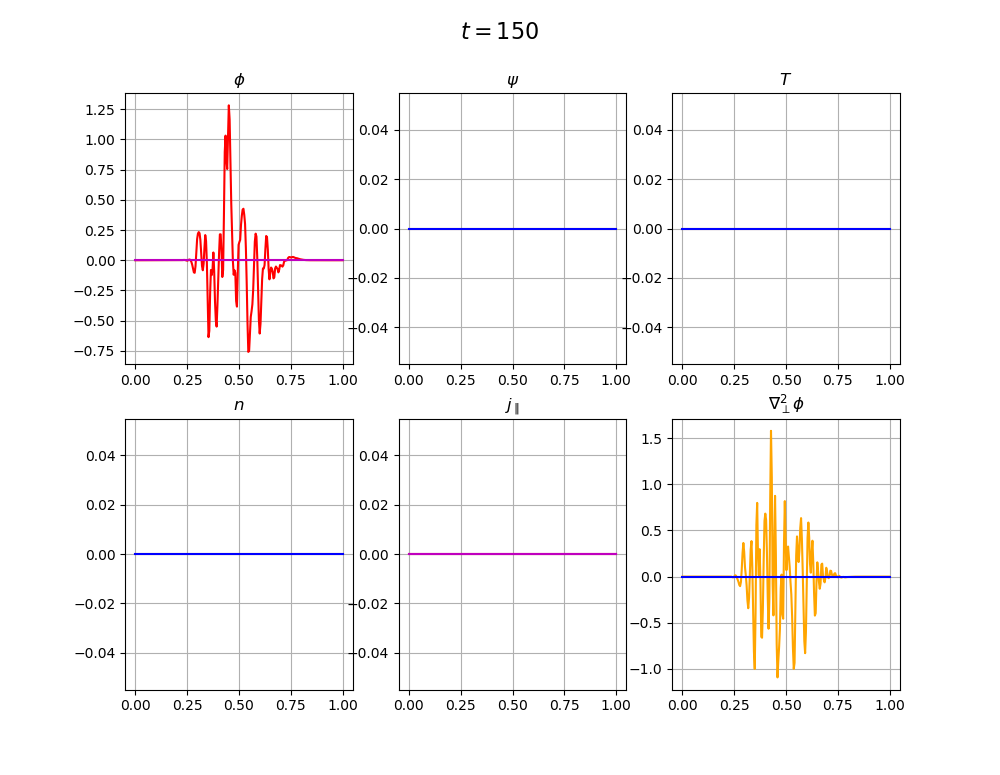
\includegraphics[width=0.7\textwidth]{./images/lw-256-150.png}
	\caption{radial mode structure with LW-256}
\end{figure}
\end{frame}	

\begin{frame}{comparision between different algorithm}
\begin{figure}[H]
	\centering
	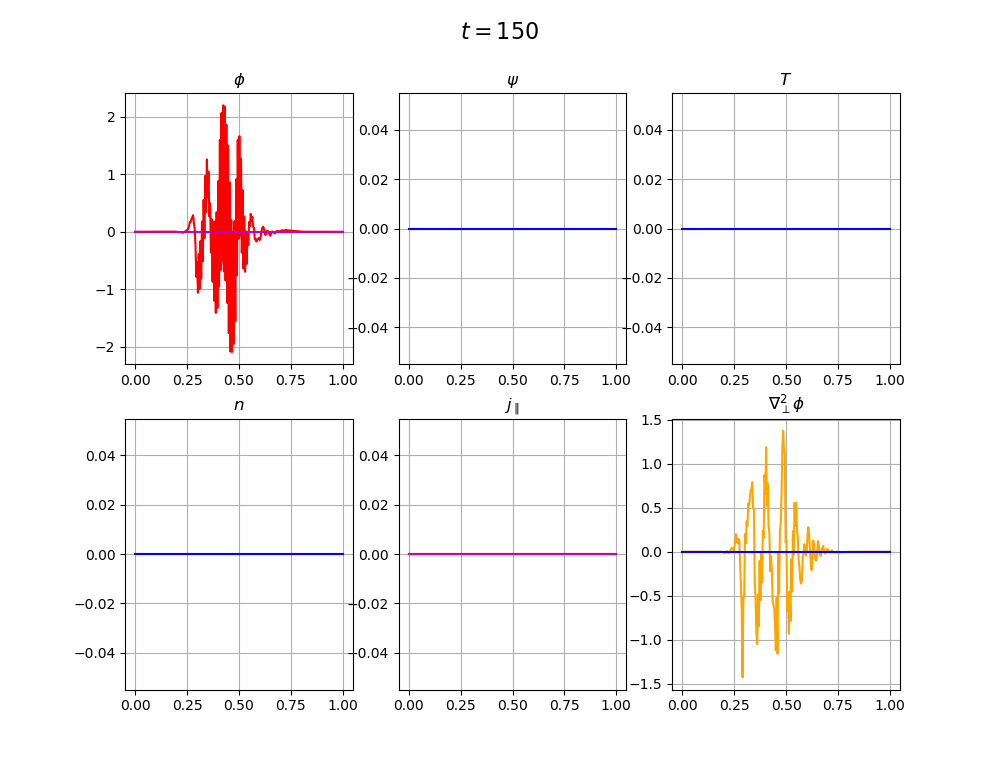
\includegraphics[width=0.7\textwidth]{./images/ab-256-150.png}
	\caption{radial mode structure with AB-256}
\end{figure}
\end{frame}	
%
%%
\begin{frame}{comparision between different algorithm}
\begin{figure}[H]
	\centering
	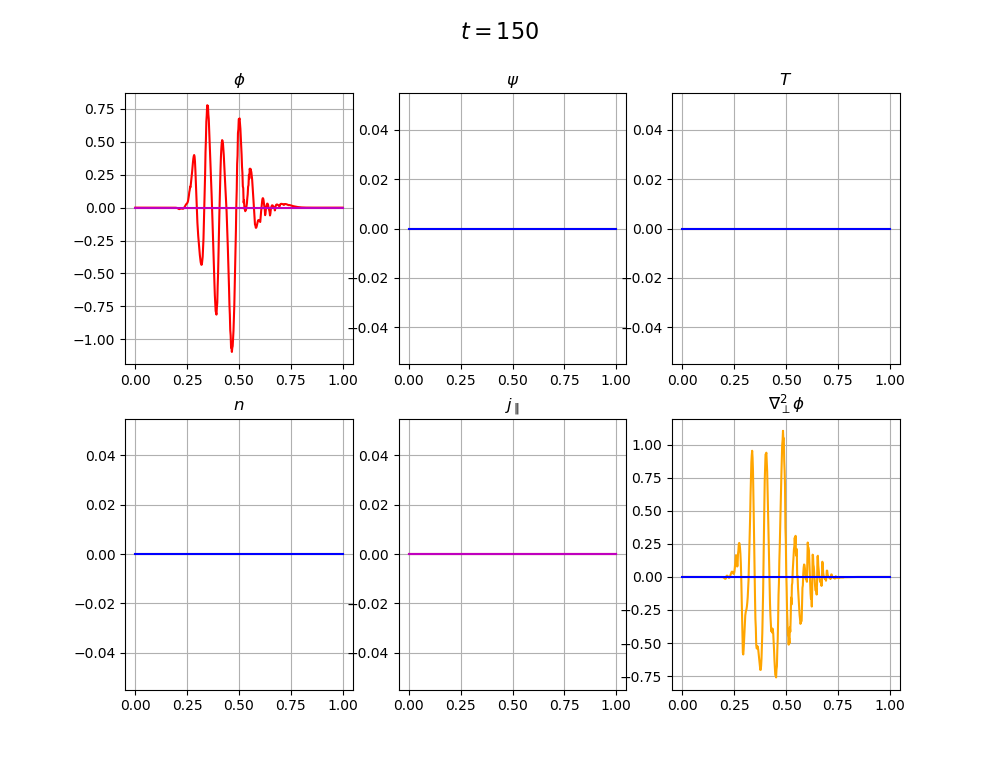
\includegraphics[width=0.7\textwidth]{./images/ab-512-150.png}
	\caption{radial mode structure with AB-512}
\end{figure}
\end{frame}	
%
%
\begin{frame}{revisiting to former simulation result}
	\begin{figure}[H]
		\centering
		\subfigure[$\beta=0.1\%$]{
			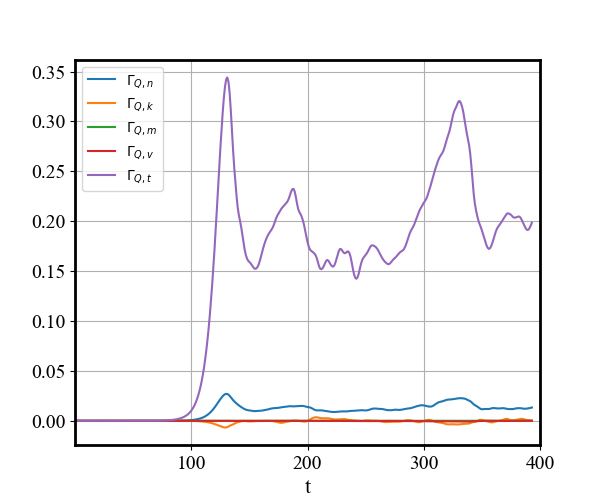
\includegraphics[width=0.4\textwidth]{../../../notes_on_energy_transfer/images/Q_tur_b01.png} 
		}
		\subfigure[$\beta=1.0\%$]{
			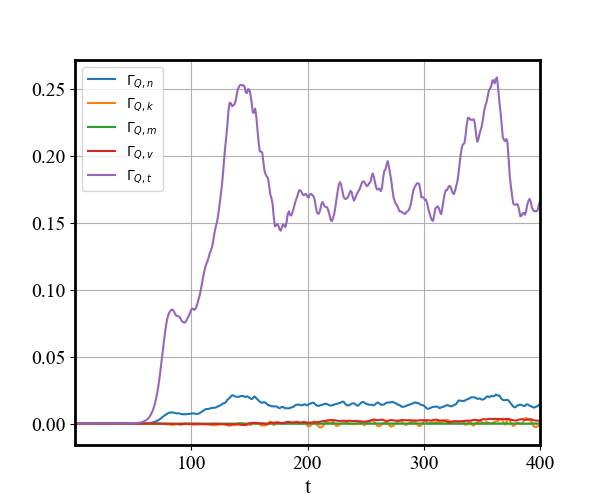
\includegraphics[width=0.4\textwidth]{../../../notes_on_energy_transfer/images/Q_tur_b10.png}
		}
		\caption{Temporal evolution of radial tansport flux}
	\end{figure}
\end{frame}
%
%
\begin{frame}{revisiting to former simulation result}
	\begin{figure}[H]
		\centering
		\subfigure[inner region]{
			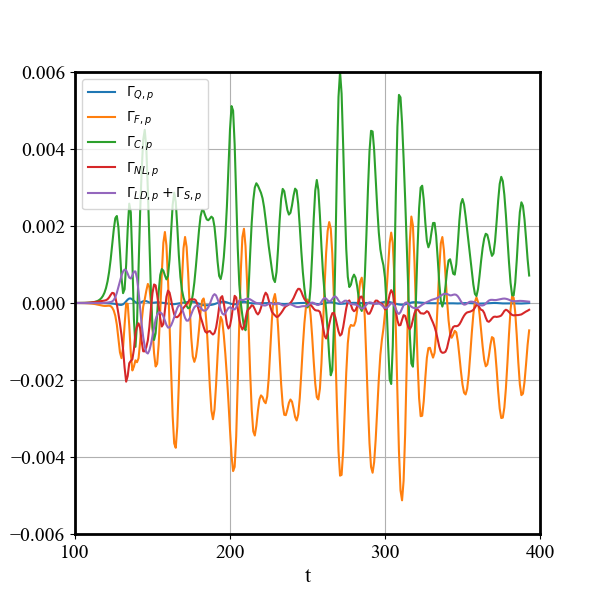
\includegraphics[width=0.4\textwidth]{../../../notes_on_energy_transfer/images/p10_b01_02-04.png} 
		}
		\subfigure[outer region]{
			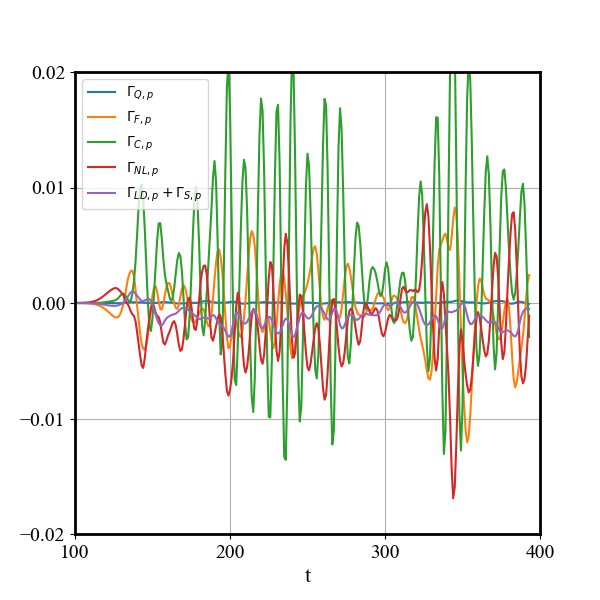
\includegraphics[width=0.4\textwidth]{../../../notes_on_energy_transfer/images/p10_b01_05-08.png}
		}
		\caption{Temporal evolution of $p_{1,0}$ energy drives with $\beta=0.1\%$}
	\end{figure}
\end{frame}
%
%
\begin{frame}{revisiting to former simulation result}
	\begin{figure}[H]
		\centering
		\subfigure[inner region]{
			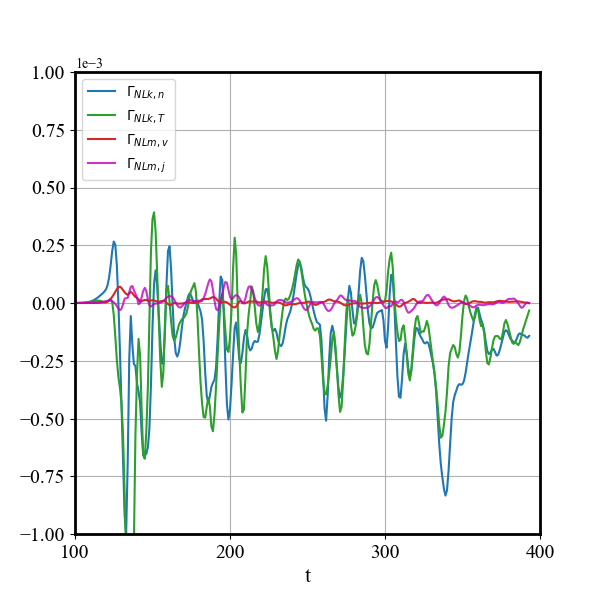
\includegraphics[width=0.4\textwidth]{../../../notes_on_energy_transfer/images/pnl_b01_02-04.png} 
		}
		\subfigure[outer region]{
			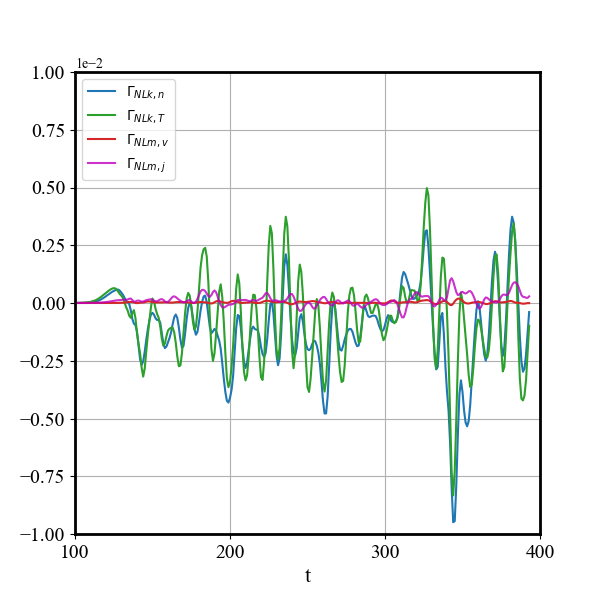
\includegraphics[width=0.4\textwidth]{../../../notes_on_energy_transfer/images/pnl_b01_05-08.png}
		}
		\caption{Temporal evolution of the component of $\Gamma_{NL,p}$}
	\end{figure}
\end{frame}

%
\begin{frame}{revisiting to former simulation result}
\begin{figure}[H]
	\centering
	\subfigure[inner region]{
		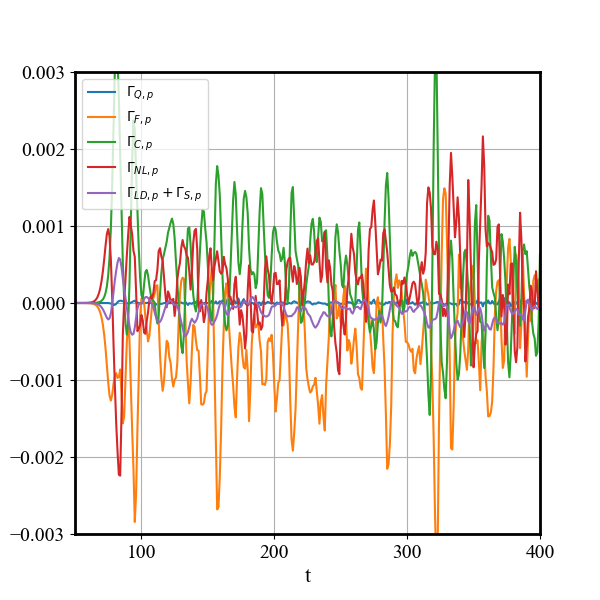
\includegraphics[width=0.4\textwidth]{../../../notes_on_energy_transfer/images/p10_b10_02-04.png} 
	}
	\subfigure[outer region]{
		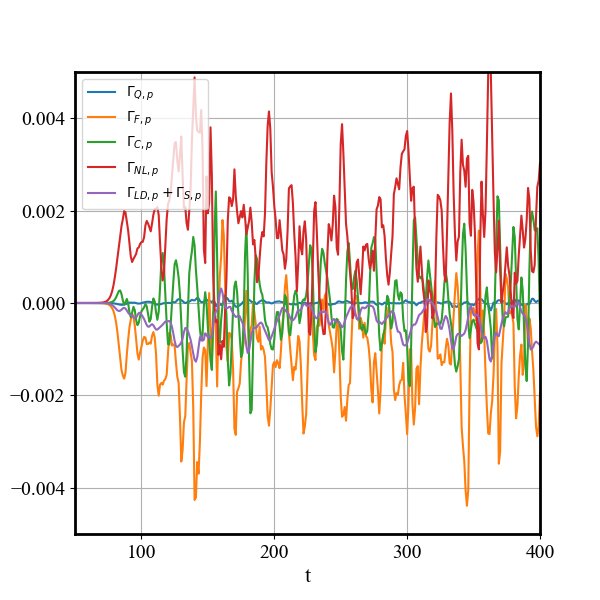
\includegraphics[width=0.4\textwidth]{../../../notes_on_energy_transfer/images/p10_b10_05-08.png}
	}
	\caption{Temporal evolution of $p_{1,0}$ energy drives with $\beta=0.1\%$}
\end{figure}
\end{frame}
%
%
\begin{frame}{revisiting to former simulation result}
	\begin{figure}[H]
		\centering
		\subfigure[inner region]{
			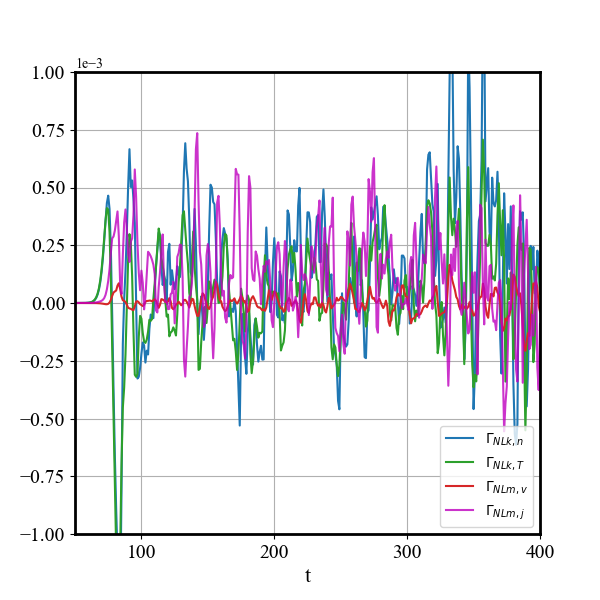
\includegraphics[width=0.4\textwidth]{../../../notes_on_energy_transfer/images/pnl_b10_02-04.png} 
		}
		\subfigure[outer region]{
			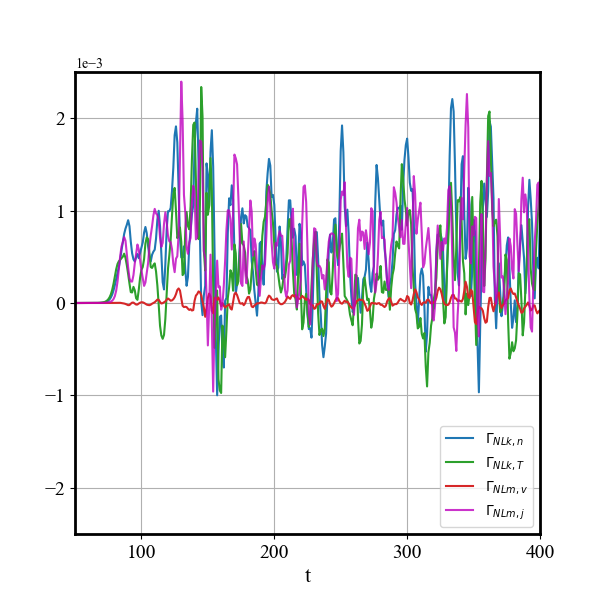
\includegraphics[width=0.4\textwidth]{../../../notes_on_energy_transfer/images/pnl_b10_05-08.png}
		}
		\caption{Temporal evolution of the component of $\Gamma_{NL,p}$}
	\end{figure}
\end{frame}
%
%
\begin{frame}{modification of energy transfer equation}
\begin{equation}
<f>=\frac{\int{f}dV}{\int{dV}}
=\frac{\int{f}\ rdrd\theta{d\zeta}}{\int\ rdrd\theta{d\zeta}}
\end{equation}

for zonal flow energy $E_k=\frac{1}{2}<v_E^2>$:
\begin{equation}
\frac{\partial}{\partial{t}}E_k=\Gamma_{NLk,k}+\Gamma_{NLm,k}+\Gamma_{C,k}
\end{equation}
for pressure $E_p=\frac{1}{2}<p^2>$:
\begin{equation}
p=p_i+p_e=n_0T+(1+\tau)T_0{n}
\end{equation}

\begin{equation}
\frac{\partial}{\partial{t}}E_p=\Gamma_{Q,p}+\Gamma_{F,p}+\Gamma_{C,p}+\Gamma_{LD,p}+\Gamma_{NL,p}+\Gamma_{S,p}
\end{equation}
\end{frame}

\begin{frame}{modification of energy transfer equation}
flux surface average
\begin{equation}
<f>=\frac{\int{f}dS}{\int{dS}}
=\frac{\int{f}\ d\theta{d\zeta}}{\int\ d\theta{d\zeta}}
\end{equation}
for zonal flow 
\begin{equation}
\frac{\partial}{\partial{t}}<v_E>
=-\frac{1}{r^2}\frac{\partial}{\partial{r}}r^2<v_\theta{v_r}>
+\frac{\beta}{n_{eq}}\frac{1}{r^2}\frac{\partial}{\partial{r}}r^2<B_\theta{B_r}>
-\frac{2\epsilon}{n_{eq}}<p\sin\theta>
\end{equation}
and in the code, we use the alternative expression,
\begin{equation}
\frac{\partial}{\partial{t}}<v_E>
=\frac{1}{r}<\phi\frac{\partial{\Omega}}{\partial\theta}>
+\frac{\beta}{n_{eq}}\frac{1}{r}<A\frac{\partial{A}}{\partial\theta}>
-\frac{2\epsilon}{n_{eq}}<p\sin\theta>
\end{equation} 
with the Fourier expansion,
\begin{equation}
\frac{\partial}{\partial{t}}<v_E>
=\sum_{m1+m2=0}{\phi_{m1}}{\Omega_{\theta,m2}}
+\sum_{m1+m2=0}{A_{m1}}{j_{\theta,m2}}
-\frac{i\epsilon}{n_{eq}}(p_{1,0}-p_{-1,0})
\end{equation} 
\end{frame}


\begin{frame}{modification of energy transfer equation}
as for equation for thr evolution of $<p\sin\theta>$
\begin{equation}
\frac{\partial}{\partial{t}}<p\sin\theta>
=<(R_Q+R_F+R_C+R_{NL}+R_{LD}+R_{S})\sin\theta>
\end{equation}

\begin{equation}
\begin{aligned}
<R_Q\sin\theta>&=
a[(1+\tau)T_{eq}\frac{\partial{n_{eq}}}{\partial{r}}+n_{eq}\frac{\partial{T_{eq}}}{\partial{r}}]<\phi\cos\theta>\\
&+(1+\tau)\beta{T_{eq}}\frac{\partial{j_0}}{\partial{r}}<A\cos\theta>\\
<R_F\sin\theta>&=
(\Gamma+\tau)n_{eq}T_{eq}\frac{\epsilon}{q}<v\cos\theta>
-(1+\tau)T_{eq}\frac{\epsilon}{q}<j\cos\theta>	\\
<R_C\sin\theta>&=
\epsilon(\Gamma+\tau)p_{eq}<v_\theta>	\\
&+\epsilon(2\Gamma-1)p_{eq}<\frac{\partial{T}}{\partial{r}}>
+\epsilon((\Gamma-1)-\tau(\tau+1))T_{eq}^2<\frac{\partial{n}}{\partial{r}}>	\\
<R_{LD}\sin\theta>&=
-(\Gamma-1)\sqrt{\frac{8T_{eq}}{\pi}}n_{eq}\frac{\epsilon}{q}<T\sin\theta>	\\
\end{aligned}
\end{equation}
\end{frame}	
%
%
%
%
\begin{frame}{Residual zonal flow}
\begin{itemize}
	\item gyrofluid simulation [Beer,Waltz]: a total collisionless decay of poloidal rotation
	\item gyrokinetic analysis by [RH 1998]: linear collisionless kinetic mechanisms do not damp the zonal flows completely
	\item verification by various gyrokinetic codes
	\item considering shaping effect [Xiao 2006]
	\item modification of zonal flow closures in gyrofluid model[Mandell,Sugama]
\end{itemize}
\end{frame}

\begin{frame}{Residual zonal flow }
Considering the polarization drift in plasma, 
\begin{equation}
v_{pj}=\frac{m_j}{e_jB^2}\frac{d\pmb{E}}{dt}
\end{equation}
this gives rise to the polarization current,
\begin{equation}
j^{cl}=\sum_{j}{e_jn_j\pmb{v}_{pj}}=\epsilon_0\epsilon^{cl}\frac{d\pmb{E}}{dt}
\end{equation}
where $\epsilon^{cl}=m_in_i/\epsilon_0B^2=(\omega_{pi}/\Omega_i)^2=(k_{Di}\rho_i)^2>>1$
\end{frame}

\begin{frame}{Residula zonal flow}
And in tokamak, considering the toroidal effect, we should include the traped and passing particals. Some fraction of charged particals($f_t\sim\sqrt{\epsilon},\epsilon=r/R$) are trapped by the magnetic mirror and have a radial excursion by 
\begin{equation}
\Delta_t=\sqrt{\epsilon}\rho_{pi}=\frac{q\rho_i}{\sqrt{\epsilon}}
\end{equation}
and as for passing partical the excursion is
\begin{equation}
\Delta_p=q\rho_i
\end{equation}
\end{frame}


\begin{frame}{Residula zonal flow}
So during this trapped partial orbit motion, we alse have the similar polarization effect if we have radial electric field $E_r$, 
\begin{equation}
j^{nc}=\epsilon_0\epsilon^{nc}\frac{dE_r}{dt}
\end{equation}
\begin{equation}
\epsilon^{nc}=\sqrt{\epsilon}k_{Di}^2\Delta_t^2=\frac{q^2}{\sqrt{\epsilon}}\epsilon^{cl}
\end{equation}
and Hinton-Rosenbluth give a expression for the polarization as,
\begin{equation}
\epsilon=\epsilon^{cl}+\epsilon^{nc}=\frac{\omega_{pi}^2}{\Omega_i^2}(1+\frac{1.6q^2}{\sqrt{\epsilon}})
\end{equation}
The factor 1.6 comes from detialed kinetic calculation including passing partical contribution.
\end{frame}

\begin{frame}{Residula zonal flow}
Then we consider the continuity equation of the polarization current,
\begin{equation}
\frac{\partial\rho_p}{\partial{t}}+\nabla\cdot\pmb{j}_p=S		
\end{equation}
$S$ is the external source density.Taking the flux surface average and Fourier expansion in space, 
\begin{equation}
\frac{\partial}{\partial{t}}<\rho_p(\pmb{k})>+<i\pmb{k}_\perp\cdot{\pmb{j}_p}(\pmb{k})>=<S(\pmb{k})>
\end{equation}
\begin{equation}
\epsilon_0\epsilon_p<k_\perp^2>\Phi_k=<\rho_p>-\int<S(\pmb{k})>dt
\end{equation}
\end{frame}


\begin{frame}{Residula zonal flow}
Consider an initial source perturbation $<S(\pmb{k})>=\delta_k(0)\delta(t)$. when the time scale is in a few gyro motion and much shorter than the bounce time of trapped partical.we have,
\begin{equation}
\epsilon_0\epsilon^{cl}\Phi_k(t=+0)=-e_i\delta{n_k(0)}
\end{equation} 
when the time scale is longer than the bounce time of trapped particals, the electrostatic potential is further shielded by the addition of the neoclassical polarization, then we have,
\begin{equation}
\epsilon_0(\epsilon^{cl}+\epsilon^{nc})\Phi_k(t=+\infty)=-e_i\delta{n_k(0)}
\end{equation}
Therefore, the ratio of the long term zonal flow potential to the initial zonal flow potential is given by, 
\begin{equation}
\frac{\Phi_k(t=\infty)}{\Phi_k(t=0)}=\frac{\epsilon^{cl}}{\epsilon^{cl}+\epsilon^{nc}}
\end{equation}
Using the Hinton formula, we have,
\begin{equation}
\frac{\Phi_k(t=\infty)}{\Phi_k(t=0)}=\frac{1}{1+1.6q^2/\sqrt{\epsilon}}
\end{equation}
\end{frame}


\begin{frame}{Geodesic acoustic mode}
\begin{itemize}
\item first prediction by [Winsor 1968]
\item Fully forgotten between 1968 and 1996
\item dispersion relation, frequency, radial structure and propagation
\item close relation to alfven eigen mode
\item experimental observations of GAM, H1-heliac,[Shats PRL 2002]; DIII-
D, [McKee PoP 2003]
\end{itemize}
\end{frame}

\begin{frame}{Geodesic acoustic mode}
The starting equations are the follows:
\begin{equation}
\begin{aligned}
&\rho_0\frac{\partial{\pmb{v}}}{\partial{t}}=\frac{1}{c}\pmb{J}\times\pmb{B}-\nabla{p}	\\
&\frac{\partial\rho}{\partial{t}}+\nabla\cdot\rho_0\pmb{v}=0	\\
&\nabla\phi=\frac{1}{c}\pmb{b}\times\pmb{B}	\\
&\nabla\cdot\pmb{J}=0	\\
&\rho_0^{-\gamma}-\gamma{p_0}\rho_0^{-\gamma-1}\frac{\partial{\rho}}{\partial{t}}+\pmb{v}\cdot\nabla({p_0}\rho_0^{-\gamma})=0
\end{aligned}
\end{equation}	
\end{frame}

\begin{frame}{Geodesic acoustic mode}
finally, we can deduce the dispersion relation:
\begin{equation}
\begin{aligned}
& \omega^2\int{|\rho|^2}\mathcal{J}dS= \\ 
& \frac{\gamma{p_0}}{\rho_0}( |\int\rho_0\frac{\pmb{B}\times\nabla\psi\cdot\nabla{B^2}}{B^4}\mathcal{J}dS|^2/\int\frac{|\nabla\psi|^2}{B^2}\mathcal{J}dS + \int\frac{|\pmb{B}\cdot\nabla\rho|^2}{B^2}\mathcal{J}dS )
\end{aligned}
\end{equation}
The first term is due to motion in the $\pmb{B}\times\nabla\psi$direction.It is associated with geodesic curvature, i.e., the surface component of the magnetic field line curvature. And the second \textbf{ordinary sound propagation propagating along the field lines}.
\end{frame}


\begin{frame}{Geodesic acoustic mode}
In the limit of circular cross section with large aspect ratio($r\ll R$), the dispersion relation becomes,
\begin{equation}
\omega^2=\frac{2\gamma{p_0}}{\rho_0{R}^2}[1+1/(2q^2)]=2\frac{C_s^2}{R^2}(1+1/(2q^2))
\end{equation}
with the defination of sound wave velocity in neutral gas $C_s=(\gamma{p_0}/\rho_0)^{1/2}$ .

\begin{quote}
{\color{magenta} question: relation between RHF and GAM}
\end{quote}

\end{frame}





\end{document}